
\documentclass{exam}

\usepackage{fullpage}
\usepackage{enumitem}
\usepackage{siunitx} 
\usepackage{graphicx}
\usepackage[fleqn]{amsmath}
\usepackage{cancel}
\usepackage{polynom}
\usepackage{float}
\usepackage{mdwlist}
\usepackage{booktabs}
\usepackage{cancel}
\usepackage{polynom}
\usepackage{caption}

\newcommand{\degree}{\ensuremath{^\circ}} 
\everymath{\displaystyle}

% \begin{figure}[H]
%   \centering
%   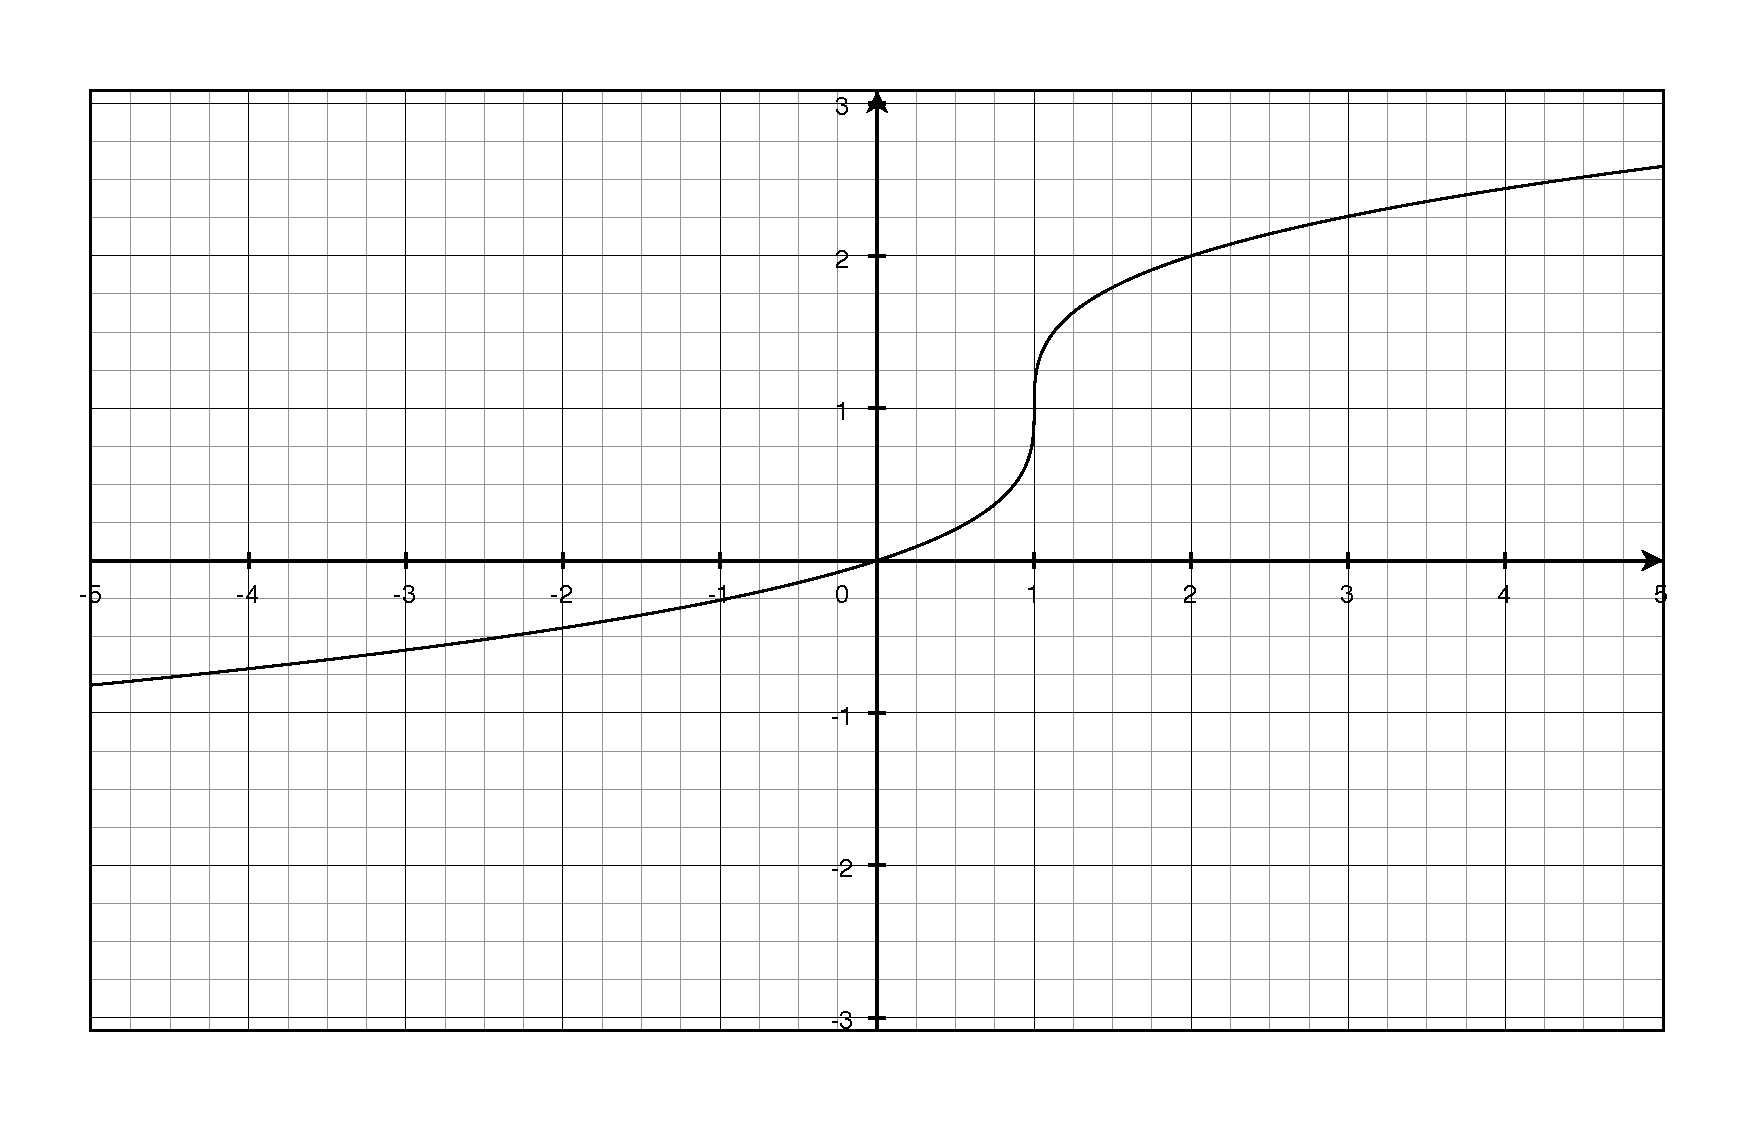
\includegraphics[scale=.3]{question7.eps}
%   \caption*{Question 7}
% \end{figure}

% \begin{tabular}{cc}
% \toprule
% period & amplitude \\
% \midrule
%   $\pi$ & $2$ \\
% \bottomrule
% \end{tabular}

% \textwidth 6.5 in

% \printanswers

\ifprintanswers 
\usepackage{2in1, lscape} 
\fi

\title{Math 263a \\ Practice Problems Week Three}
\date{February 1, 2012}

\begin{document}

\maketitle

\section{Finding Limits}
For questions \ref{limit:first} to \ref{limit:last}, find each limit.

\begin{enumerate}

\item
\label{limit:first}
\[
  \lim_{x \to 5} \frac{x + 2}{x - 4}
\]

\item
\[
  \lim_{x \to 1} \frac{x^2 - x}{2x^2 + 5x - 7} 
\]

\item
\[
  \lim_{x \to -3} \frac{x^2 - x - 12}{x^2 + 4x + 3}
\]

\item
\label{limit:last}
\[
  \lim_{x \to 4} \frac{x^2 - 16}{\sqrt{x} - 2}
\]

\end{enumerate}
\section{Proving Limits}

For questions \ref{proof:first} to \ref{proof:last}, give an $\epsilon$/$\delta$ proof of each limit.

\begin{enumerate}[resume]
\item
\label{proof:first} 
\[
  \lim_{x \to -3} (2x + 1) = -5
\]

\item
\[
  \lim_{x \to 0} \frac{3x^2 + x}{x} = 1
\]

\item
\label{proof:last}
\[
  \lim_{x \to 2} \frac{x^2 - 4}{x-2} = 4
\]

\end{enumerate}

\end{document}

